\section{Magnetorquer model}

%\nomenclature[Sncoil]{$n_{coil}$}{The number of windings of the coil}
%\nomenclature[SIcoil]{$I_{coil}$}{The electric current flowing through the coil}
%\nomenclature[SAcoil]{$\vec A_{coil}$}{The vector perpendicular to the cross-sectional area of the magnetorquer}
\nomenclature[Sm]{$\vec m_{mt}$}{The magnetic dipole moment}

Since the primary actuators are chosen to be reaction wheels, a configuration of three magnetorquers orthogonal and doubled will be used for desaturation of the reaction wheels.  

Having a solenoid onboard of the satellite, referred as a magnetorquer through which the current could be controlled and hence the dipole moment.

The interaction of the dipole with the magnetic field of the Earth will result in a torque that will be perpendicular to the magnetic field vector according to the following equation \cite{SADC}:
\begin{flalign}
   \vec N_{mt} = \vec m_{mt} \times \vec B
	\label{eq:NT}
\end{flalign} 
where $\vec N$ is the torque produce by the magnetorquer and will be the torque that will influence the satellite dynamics, $\vec B$ is the vector of the magnetic field of the Earth and $\vec m_{mt} $ is the magnetic dipole moment generated by the magnetorquer.

The magnetic moment $\vec m_{mt}$ is given by \cite{MagMom}:
\begin{flalign}
	\vec m_{mt} = n_{coil} \ I_{coil} \ \vec A_{coil}
	\label{eq:mm}
\end{flalign} 
where $n_{coil}$ is the windings of the coil, $I_{coil}$ is the electric current through the coil and $\vec A_{coil}$ is the vector perpendicular to the cross-sectional area of the magnetorquer.

Using \ref{eq:NT} and \ref{eq:mm} and taking the magnitude, the applied torque on the satellite is \cite{SJ}:
\begin{flalign}
	\vec N_{mt} = n_{coil} \ \rvert I_{coil}\rvert \ \rvert \vec A_{coil}\rvert \ |\vec B| \sin (\theta)
	\label{eq:ft}
\end{flalign} 
where $\sin (\theta)$ is the angle between the plane $A_{coil}$ and the magnetic field vector $\vec B$.

Furthermore, the resistance of the magnetorqer which is a function of the temperature of the coil given as an input, can be computed as
\begin{flalign}
R_{mt} = \dfrac{nC  \rho_{mt} }{A_{wire}} = \dfrac{nC \rho_0(1+\alpha_0(T_{mt} - T_0))}{A_{wire}}
\label{eq:rt}
\end{flalign} 
where \\
$R_{mt}$ is the resistance of the magnetorquer \\
$n$ is the number of windings \\ 
$C$ is the wire circumference  \\
$A_{wire}$ is the wire cross-sectional area  \\
$\rho_0$ is the resistivity of copper  \\
$\alpha_0$ is the coefficient of resistivity temperature   \\
$T_{mt}$ is the temperature given as an input   \\
$T_0$ is the resistivity base temperature  

Using the computed resistance the current is found by dividing the voltage by the resistance of the magnetorquer. Next, in order to find the magnetic moment $m$, the current is multiplied by the number of windings and the area of the wire. For finding the torque that acts on the satellite, the magnetic moment is multiplied by the coil normal and a cross-product is used between this multiplication and the magnetic field of the Earth.

The design of the magnetorquer is described in appendix \ref{chap:F}.

\subsection{Magnetorquers open-loop control}
In order to find what voltage to output for having a certain amount of torque, a gain between voltage and magnetic moment is found. For the coil model, the control signal is the voltage. Therefore, translating the magnetic moment demand to voltage is found as follows:
\begin{flalign}
\frac{\vec m_{mt}}{v} = \frac{n_{coil} \vec A_{coil} \vec I_{coil}}{R_{mt}} \mathcal {K}
	\label{eq:gain}
\end{flalign} 
\begin{flalign}
 \mathcal{K} = \frac{\vec m_{mt} R_{mt} }{ n_{coil}  \vec A_{coil} \vec I_{coil} v}
	\label{eq:gainn}
\end{flalign} 
where \\
$v$ is the voltage \\
$\mathcal {K}$ is the gain

The voltage can be found using the following transfer function:
\begin{flalign}
	\frac{I_{coil}}{v} = \frac{1}{R_{mt}}
	\label{eq:voltage}
\end{flalign} 

where the voltage is found to be $1.25 V$

The magnetorquer open loop control can be seen in figure \ref{fig:op}:
\begin{figure}[H]
	\centering
	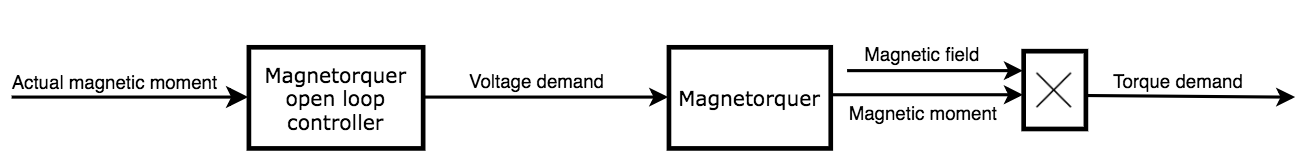
\includegraphics[width=1\linewidth]{figures/MT_open_loop}
	\caption{Magnetorquer open loop control }
	\label{fig:op}
\end{figure}

\subsection{Relation between the coil current and generated magnetic field} 
Given a current $I$ going through a coil, the interest is to find the magnetic field $B$ at a certain point located distance $r$ from the coil. Finding an estimate of the magnetic field at any point will give the possibility to change the location of the magnetometers around. For computing the magnetic field in the center of a square coil, the law of Biot-Savart is used \cite{SJ}:
\begin{flalign}
	d\vec B = \frac{\mu_0 I}{4 \pi}  \frac{d \vec s \times \hat{\vec r}}{r^2}
	\label{eq:BS}
\end{flalign} 
where \\
$\vec B$ is the magnetic field \\
$\mu_0$ is a constant called permeability of free space and is equal with $4\pi \times 10^{-7}  \ Tm/A$ \\
$I$ is the current \\
$d \vec s $ is a length element in the direction of current \\
$\hat{\vec r}$ is the direction from $d \vec s$ to a particular position \\
$r$ is the distance from $d \vec s$ to a particular position

The magnetic field $B$ at any point is directly proportional to the current $I$ that is crossing the coil. The magnetic field generated by the current from equation \ref{eq:BS} is just a small length element $d \vec s$ of the coil. For finding the total magnetic field, all small elements need to be summed up and for this the magnetic field $B$ have to be evaluated by integrating equation \ref{eq:BS}. It is assumed that the magnetorquer coil it has a square shape and the magnetometer is placed in the middle.
